\documentclass[10pt]{beamer}
\usetheme{Feather}
\usepackage[T1]{fontenc}
\usepackage[utf8]{inputenc}
\usepackage[spanish]{babel}
\usepackage{mathrsfs}
\usepackage{amsmath}
\usepackage{amssymb}
\usepackage[utf8]{inputenc}
\usepackage[T1]{fontenc}
\usepackage{multirow}
\usepackage{multicol}
\usepackage{xcolor}
\usepackage{ragged2e}
 
\setbeamerfont{block body}{size=\small}
\title{Proyecto Final }
\subtitle{Lógica para ciencias de la computación}
\author{Salome Viana y Juanita Gómez}
\begin{document}
{\1
\begin{frame}[plain,noframenumbering]
  \titlepage 
\end{frame}}
%% 1
\begin{frame}{1. Planteamiento del Problema}
\begin{block}{Teorema de los 4 colores}
Dado cualquier mapa geográfico con regiones continuas, este puede ser coloreado con cuatro colores diferentes, de forma que no queden regiones adyacentes con el mismo color.
\end{block}
\begin{multicols}{2}
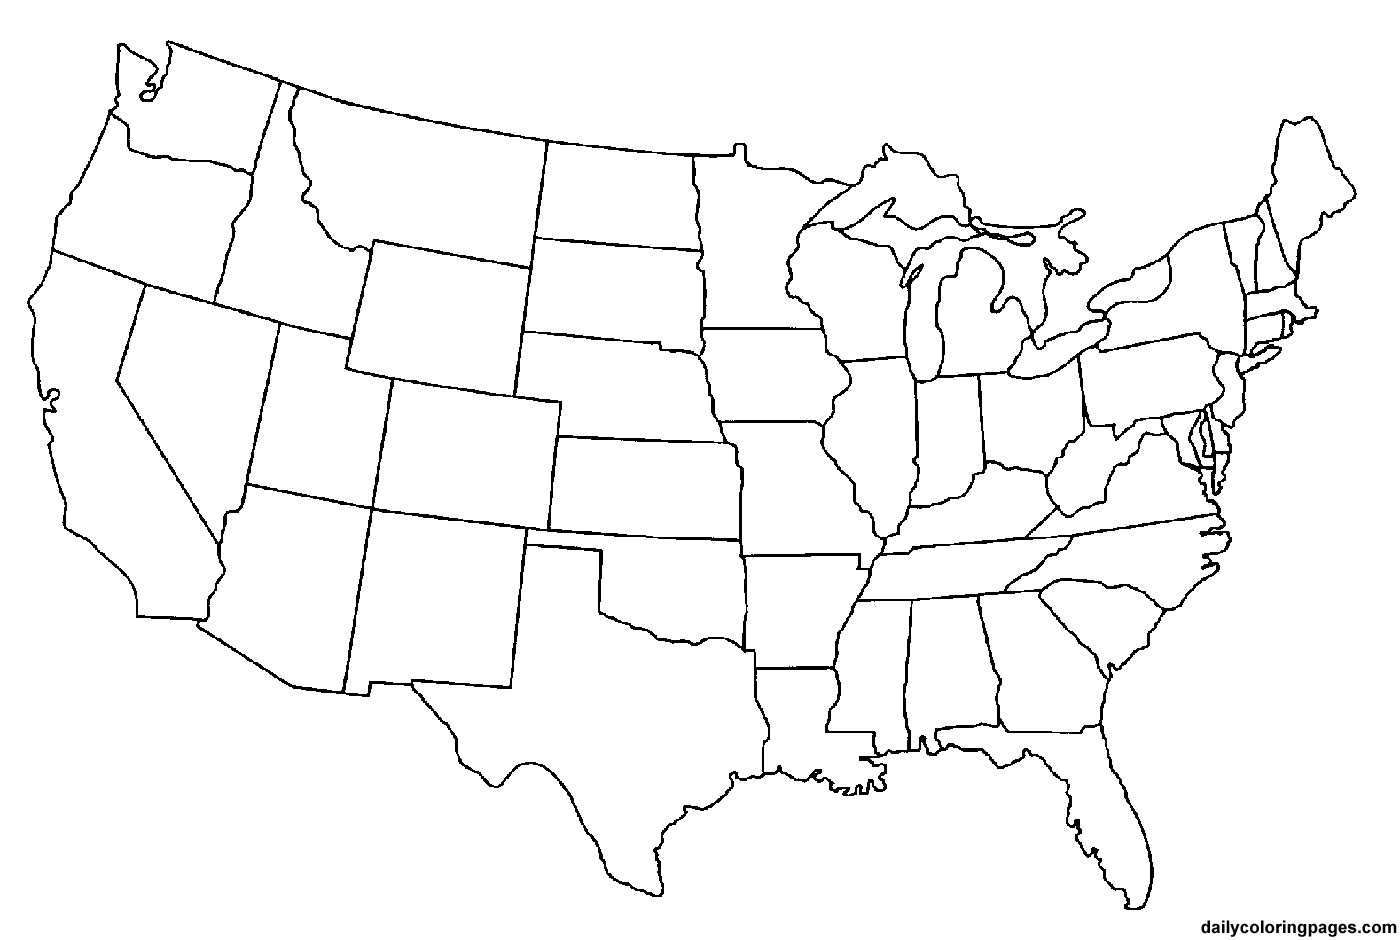
\includegraphics[scale=0.105]{Images/Mapa1.png}
\begin{itemize}
\item Dos regiones son adyacentes si comparten un segmento de frontera en común, no una esquina donde se encuentran 3 o más regiones.
\item Todas las regiones del mapa son conexas y contiguas, es decir no pueden estar divididas en 2 o más regiones.
\end{itemize}
\end{multicols}
\end{frame}

%% 2
\begin{frame}{Problema}
\begin{block}{Formulación del problema}
\justify Dado un mapa determinado, se quiere encontrar una coloración del mismo, de tal manera que no haya regiones continuas con el mismo color, usando únicamente 4 colores. 
\end{block}
\begin{multicols}{2}
\textbf{Ejemplo:}
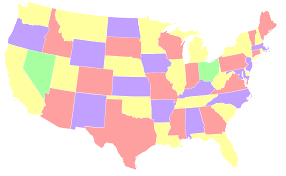
\includegraphics[scale=0.53]{Images/Mapa2.png}
\begin{itemize}
\item  \justify En la figura, se puede observar cómo el mapa de Estados Unidos está coloreado con 4 colores distintos de tal manera que se cumplen las condiciones del problema.
\end{itemize}
\end{multicols}
\end{frame}

%% 3
\begin{frame}{2. Representación en Logica proposicional}
Considere el siguiente mapa con 9 regiones. 
\begin{multicols}{2}
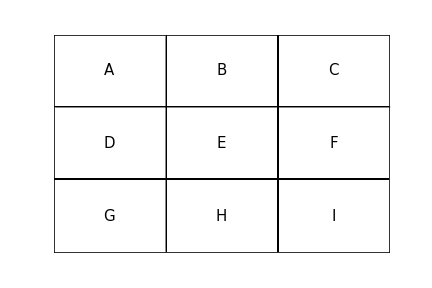
\includegraphics[scale=0.35]{Images/Mapa3.png}
\begin{itemize}
\item \justify En este mapa vamos a identificar las zonas con las letras A, B, C, D, E, F, G, H e I como se muestra en la figura.
\item  \justify Vamos a utilizar los colores \textcolor{purple}{morado}, \textcolor{orange}{naranja}, \textcolor{blue}{azul} y \textcolor{red}{verde}
\end{itemize}
\end{multicols}
\end{frame}

%% 4
\begin{frame}{Letras Proposicionales}
\justify Para este problema, las letras proposicionales van a representar las posibles coloraciones de cada una de las regiones del mapa. Por ejemplo, las 36 letras proposicionales correspondientes a este mapa serían de la siguiente manera:

\begin{itemize}
\begin{multicols}{2}
\item \textbf{a}: A esta coloreada de \textcolor{purple}{morado}.
\item \textbf{b}: A esta coloreada de \textcolor{orange}{naranja}.
\item \textbf{c}: A esta coloreada de \textcolor{blue}{azul}.
\item \textbf{d}: A esta coloreada de \textcolor{green}{verde}.
\item \textbf{e}: B esta coloreada de \textcolor{purple}{morado}.
\item \textbf{f}: B esta coloreada de \textcolor{orange}{naranja}.
\item \textbf{g}: B esta coloreada de \textcolor{blue}{azul}.
\item \textbf{h}: B esta coloreada de \textcolor{green}{verde}.
\item \textbf{i}: C esta coloreada de \textcolor{purple}{morado}.
\item \textbf{j}: C esta coloreada de \textcolor{orange}{naranja}.
\item \textbf{k}: C esta coloreada de \textcolor{blue}{azul}.
\item \textbf{l}: C esta coloreada de \textcolor{green}{verde}.
\end{multicols}

\end{itemize}
\end{frame}
\begin{frame}
\begin{itemize}
\begin{multicols}{2}
\item \textbf{m}: D esta coloreada de \textcolor{purple}{morado}.
\item \textbf{n}: D esta coloreada de \textcolor{orange}{naranja}.
\item \textbf{o}: D esta coloreada de \textcolor{blue}{azul}.
\item \textbf{p}: D esta coloreada de \textcolor{green}{verde}.
\item \textbf{q}: E esta coloreada de \textcolor{purple}{morado}.
\item \textbf{r}: E esta coloreada de \textcolor{orange}{naranja}.
\item \textbf{s}: E esta coloreada de \textcolor{blue}{azul}.
\item \textbf{t}: E esta coloreada de \textcolor{green}{verde}.
\item \textbf{u}: F esta coloreada de \textcolor{purple}{morado}.
\item \textbf{v}: F esta coloreada de \textcolor{orange}{naranja}.
\item \textbf{w}: F esta coloreada de \textcolor{blue}{azul}.
\item \textbf{x}: F esta coloreada de \textcolor{green}{verde}.
\end{multicols}
\end{itemize}

\end{frame}
\begin{frame}
\begin{itemize}
\begin{multicols}{2}
\item \textbf{y}: G esta coloreada de \textcolor{purple}{morado}.
\item \textbf{z}: G esta coloreada de \textcolor{orange}{naranja}.
\item \textbf{0}: G esta coloreada de \textcolor{blue}{azul}.
\item \textbf{1}: G esta coloreada de \textcolor{green}{verde}.
\item \textbf{2}: H esta coloreada de \textcolor{purple}{morado}.
\item \textbf{3}: H esta coloreada de \textcolor{orange}{naranja}.
\item \textbf{4}: H esta coloreada de \textcolor{blue}{azul}.
\item \textbf{5}: H esta coloreada de \textcolor{green}{verde}.
\item \textbf{6}: I esta coloreada de \textcolor{purple}{morado}.
\item \textbf{7}: I esta coloreada de \textcolor{orange}{naranja}.
\item \textbf{8}: I esta coloreada de \textcolor{blue}{azul}.
\item \textbf{9}: I esta coloreada de \textcolor{green}{verde}.
\end{multicols}
\end{itemize}

\end{frame}

\begin{frame}{Reglas}
De acuerdo con el planteamiento del problema podemos enunciar las siguientes reglas.
\begin{block}{Regla 1}
Todas las regiones deben estar coloreadas de un único color.
\end{block}
\textbf{\\ Ejemplo:}

$$(a \wedge -b \wedge -c \wedge -d) \lor (b \wedge -a \wedge -c \wedge -d) \lor (c \wedge -a \wedge -b \wedge -d) \lor (d \wedge -a \wedge -b \wedge -c)$$
 

\end{frame}

\begin{frame}{Reglas}
\begin{block}{Regla 2}
Dos regiones adyacentes no pueden estar coloreadas del mismo color. 
\end{block}
\textbf{\\ Ejemplo:}
\\
\begin{itemize}
\item $a \rightarrow (-e \wedge -m)$
\item $b \rightarrow (-f \wedge -n)$
\item $c \rightarrow (-g \wedge -o)$
\item $d \rightarrow (-h \wedge -p)$
\end{itemize}
\end{frame}

\begin{frame}{Regla}
\begin{block}{}
Teniendo en cuenta las dos condiciones que deben cumplirse en este problema, la regla que lo va a dirigir es la conjunción de la regla 1 y la regla 2. 
\end{block}
\end{frame}


\begin{frame}{Representación Gráfica de Soluciones}
Considere por ejemplo la siguiente interpretación: \\
\begin{block}{}
 \{'a:0', 'b:1', 'c:0', 'd:0', 'e:1', 'f:0', 'g:0', 'h:0', 'i:0','j:0', 'k:0', 'l:1',
      'm:0', 'n:0', 'o:1', 'p:0', 'q:0', 'r:0', 's:0','t:1', 'u:0', 'v:1', 'w:0', 'x:0', 'y:1', 'z:0', '0:0', '1:0', '2:0','3:1', '4:0', '5:0', '6:0', '7:0', '8:1', '-9:0'\}
\end{block}
Usando esta interpretación como ejemplo, vamos a construir una lista de literales de la siguiente manera:
Sin pérdida de generalidad,
\begin{itemize}
\item Si I(p)=0, agregamos a la lista –p
\item Si I(p)=1, agregamos a la lista p
\end{itemize}

\end{frame}
\begin{frame}{Representación Gráfica de Soluciones}
Con el procedimiento anterior, obtenemos la siguiente lista, la cual usaremos para generar su coloración correspondiente utilizando el código de Python.
\begin{block}{}

f =  ['-a', 'b', '-c', '-d', 'e', '-f', '-g', '-h', '-i','-j', '-k', 'l',
      '-m', '-n', 'o', '-p', '-q', '-r', '-s','t', '-u', 'v', '-w', '-x', 'y', '-z', '-0', '-1', '-2','3', '-4', '-5', '-6', '-7'
      , '8', '-9']
      
\end{block}

\begin{multicols}{2}


Note que en esta lista, los primeros 8 literales significan que la casilla A esta coloreada de naranja (y no de morado, ni azul, ni verde) y que la casilla B esta coloreada de morado (y no de naranja, azul ni verde). \\
Así, los 36 literales dan la siguiente coloración, la cual se obtuvo con el código de Python adjunto:

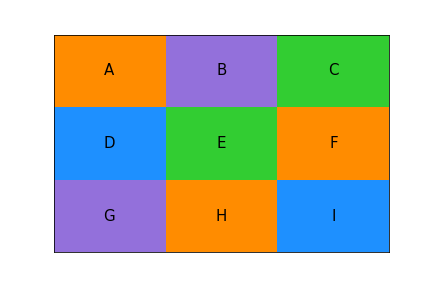
\includegraphics[scale=0.40]{Images/MapaColor.png}

\end{multicols}

\end{frame}
\begin{frame}{Resolución del problema}
\begin{itemize}
\item Creación de las reglas en lógica proposicional
\item \textbf{Tseitin}: para obtener una formula en FNC que sea igualmente buena que la regla pero más corta (y fácil de trabajar)
\item \textbf{DPLL}: para obtener una interpretación que haga verdadera la regla
\item Representación gráfica de la solución

\end{itemize}
\end{frame}
\begin{frame}{Soluciones}
\begin{multicols}{2}
Representación de la situación sin condiciones iniciales.
\center
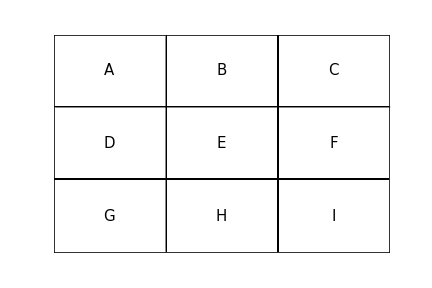
\includegraphics[scale=0.40]{Images/Mapa3.png} \\
Solución sin condiciones iniciales \\
\center
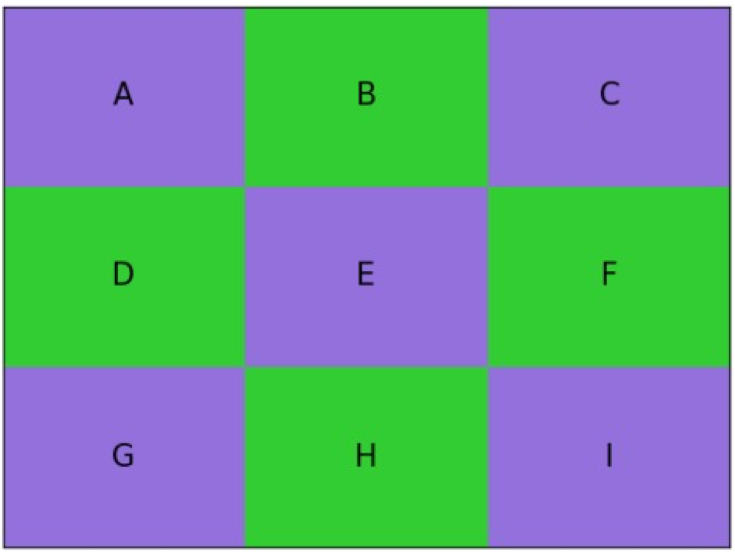
\includegraphics[scale=0.35]{Images/SinConIni.png}
\end{multicols}
\end{frame}
\begin{frame}{Soluciones}
\begin{multicols}{2}
Representación de la situación con condiciones iniciales \\
\begin{itemize}
\item r: E está coloreado de naranja
\item m: D está coloreado de morado
\item x: F está coloreado de verde
\item 8: I está coloreado de azul \\
\end{itemize}
\center
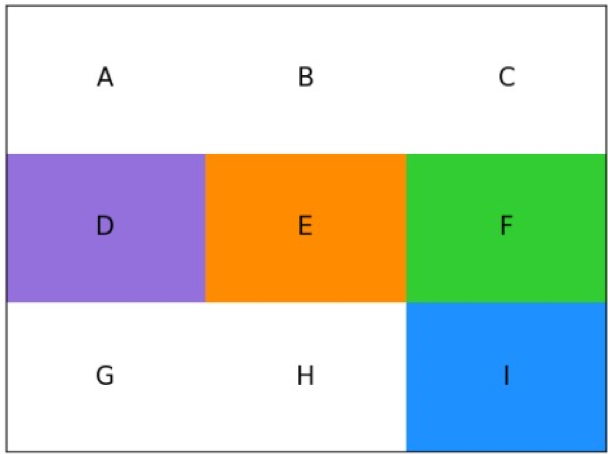
\includegraphics[scale=0.30]{Images/Picture1.png} \\
Solución sin condiciones iniciales \\
\center
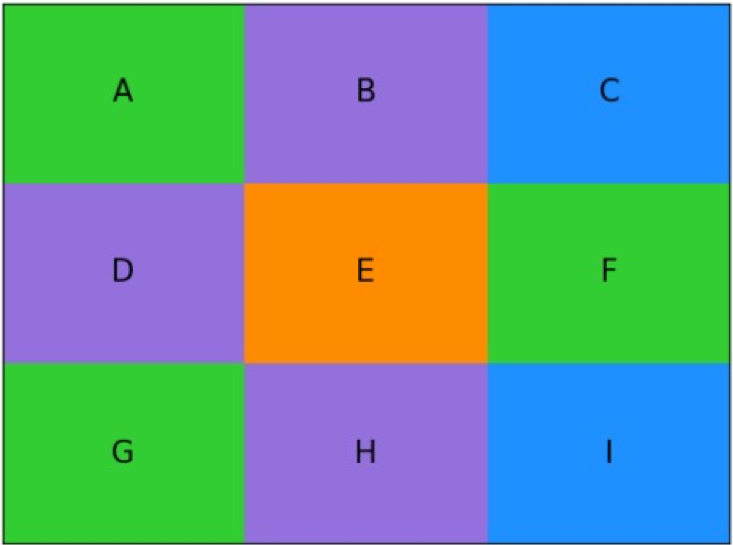
\includegraphics[scale=0.35]{Images/Picture2.png}
\end{multicols}
\end{frame}

\end{document}
